\section{REPRESENTACIONES APRENDIDAS} \label{representaciones-aprendidas}
% Distancias en ROI
\subsection{DISTANCIAS EN LA REGIÓN DE INTERÉS}
Al combinar la máscara de segmentación de posibles obstáculos con el mapa de profundidades se simplifica la tarea de calcular la distancia a estos, además al considerar sólo el trapecio delimitando el área de circulación denominada región de interés, se reducen las falsas detecciones, como se puede observar en la figura \ref{distpred}

\begin{figure}[H]
	\centering
%	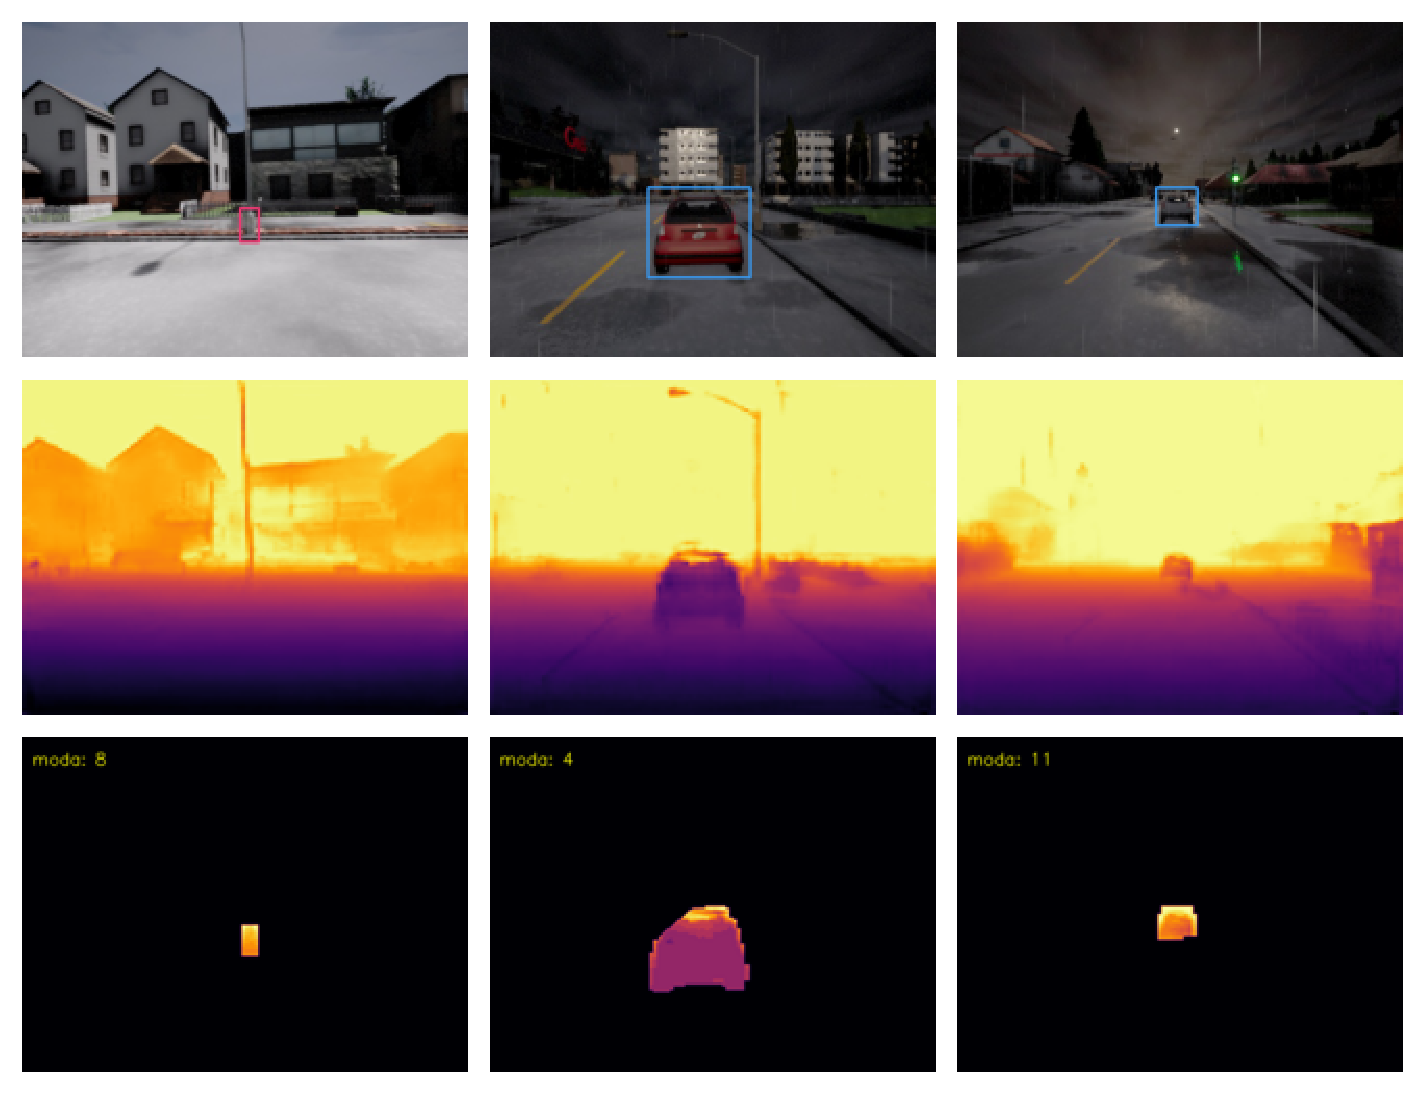
\includegraphics[scale=0.65]{imagenes/preds/distance}
	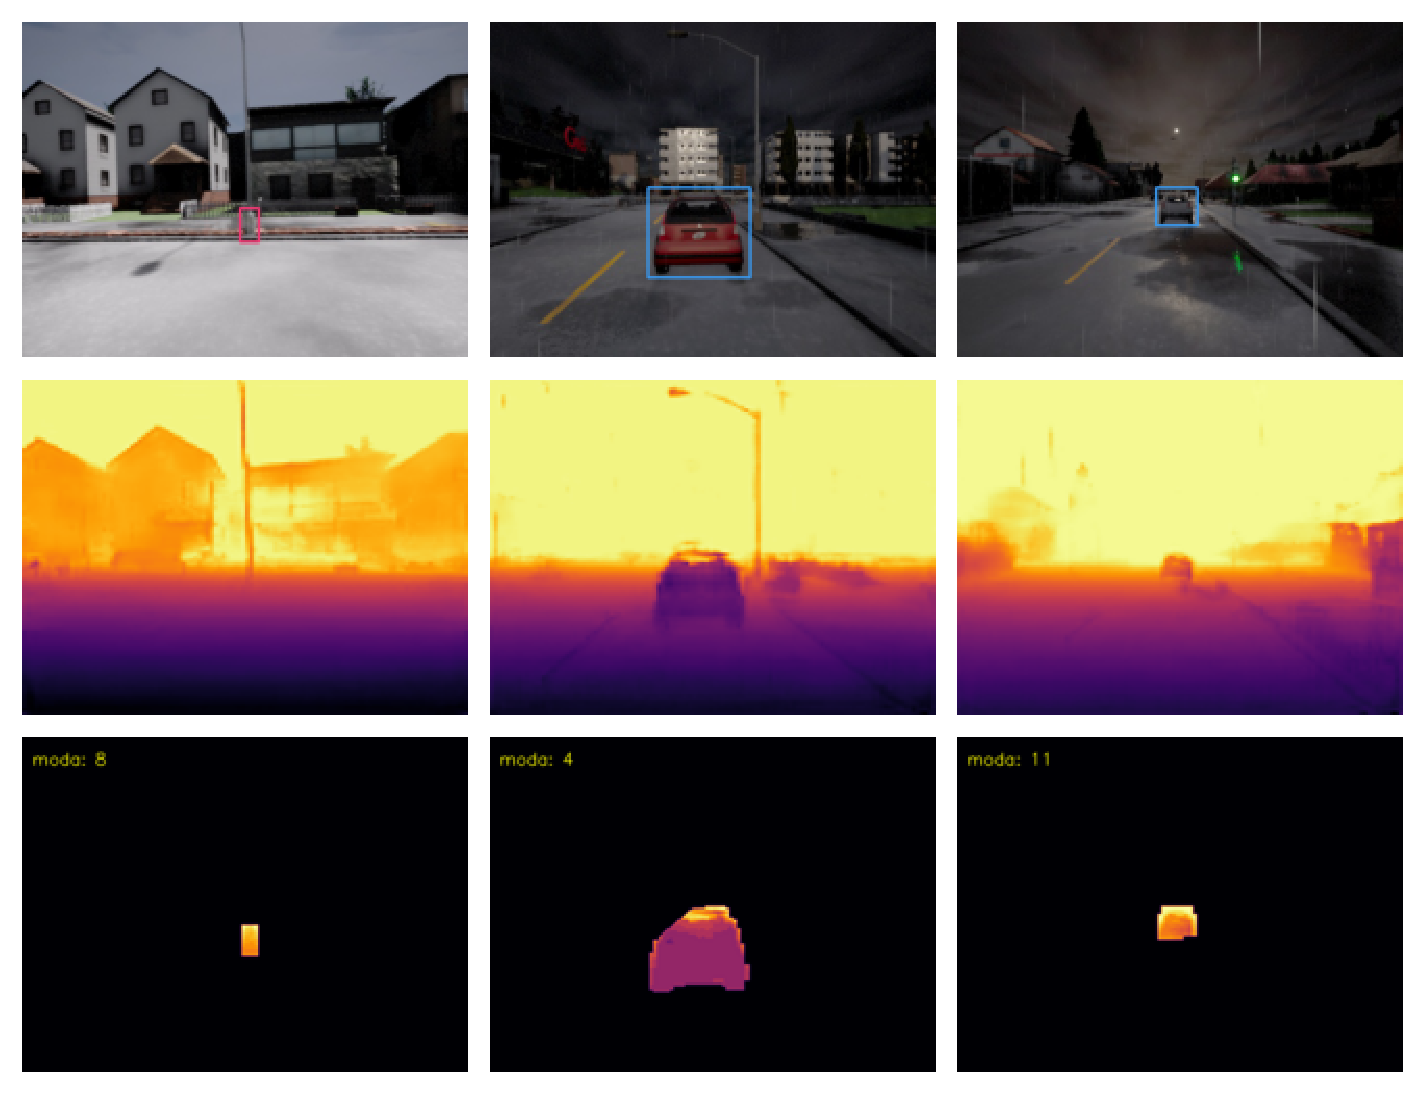
\includegraphics[scale=0.6]{imagenes/preds/distance}
	\caption[Distancia a de objetos]{distancia a objetos en el área de interés}
	\label{distpred}
\end{figure}

en la primera fila se tienen las detecciones generales usando las máscaras de segmentación, en la segunda los mapas de profundidad, y en la tercera la distancia estimada solamente a los posibles obstáculos, esta distancia general se calcula mediante la moda del valor de los píxeles del mapa de profundidades, así en cuanto un objeto está cerca, la mayoría de sus píxeles tendrán un valor bajo, siendo el límite de 4 metros a partir de la cual se empieza a frenar.

\subsection{VISUALIZACIÓN DE ZONAS DE INTERÉS}
% ScoreCam
Con el fin de comprender gráficamente a qué partes de la imagen la red neuronal de conducción presta atención durante la predicción del giro, se aplica el algoritmo scorecam, del cual se obtiene un mapa de calor que une a la imagen original, y cuyos valores altos indican mayor atención en la región.

\begin{figure}[H]
	\centering
	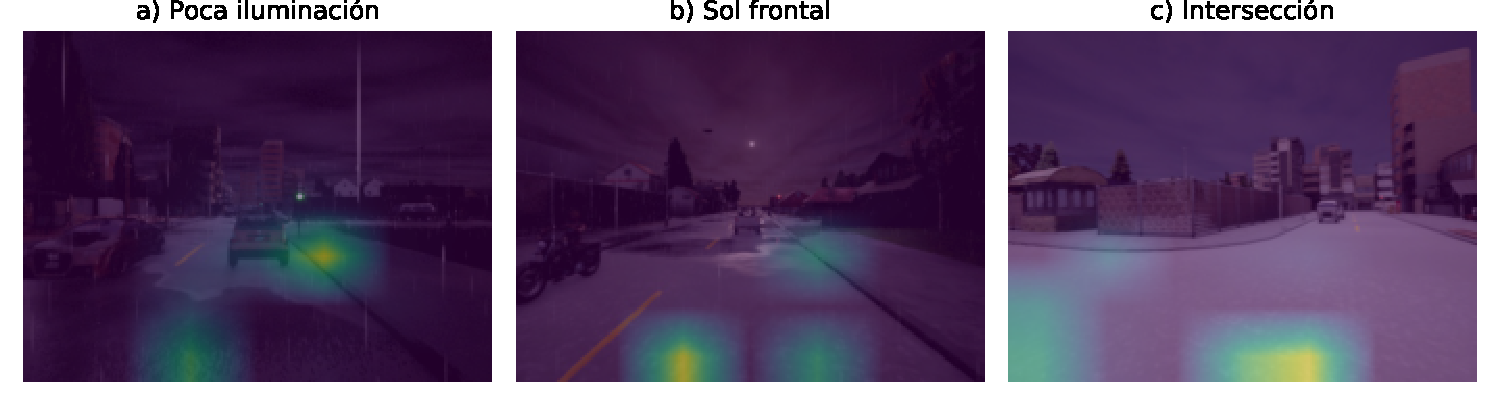
\includegraphics[scale=0.6]{imagenes/preds/scorecam}
	\caption[Regiones de Interés en la Inferencia de Dirección]{regiones de interés en la inferencia de dirección}
	\label{scorecampred}
\end{figure}

En la figura \ref{scorecampred} se observan en los casos $a$ y $b$ que aparte de la atención en el asfalto, debido a que se comparten los filtros para la inferencia de aceleración, se fija en la acera derecha, mientras que en la imagen $c$, al no tener una acera en el lado esperado se centra en la que está al frente, en la nueva calle a incorporarse.